% !TeX spellcheck = en_GB
\chapter{Results}

\section{Conventional polarisation microscopy}
\label{sec:conventional pol}

SiR has been reported to be suitable for STED microscopy with excitation at 640~nm and depletion at 775~nm \cite{DEste2015}, so one would expect the SiR-actin stained sample to behave well in the setup too. The effect of the depletion laser (in conventional, i.e.~donut mode) is presented in Figures \ref{fig:ssted} and \ref{fig:ssted supplementary}. When zoomed in (\autoref{fig:ssted supplementary}), it becomes visible that the fibres are not uniformly stained as individual fluorophores become apparent.

\begin{figure}
	\centering
	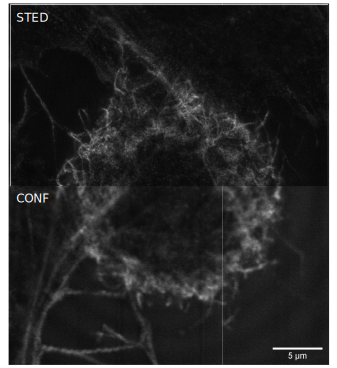
\includegraphics{ssted_2.pdf}
	\caption{
	 stained with SiR-actin, in confocal mode (bottom) and with the STED laser at 15\% power (top). More FOVs are displayed in \autoref{fig:ssted supplementary}.
	}
	\label{fig:ssted}
\end{figure}



\begin{figure}
	\centering
	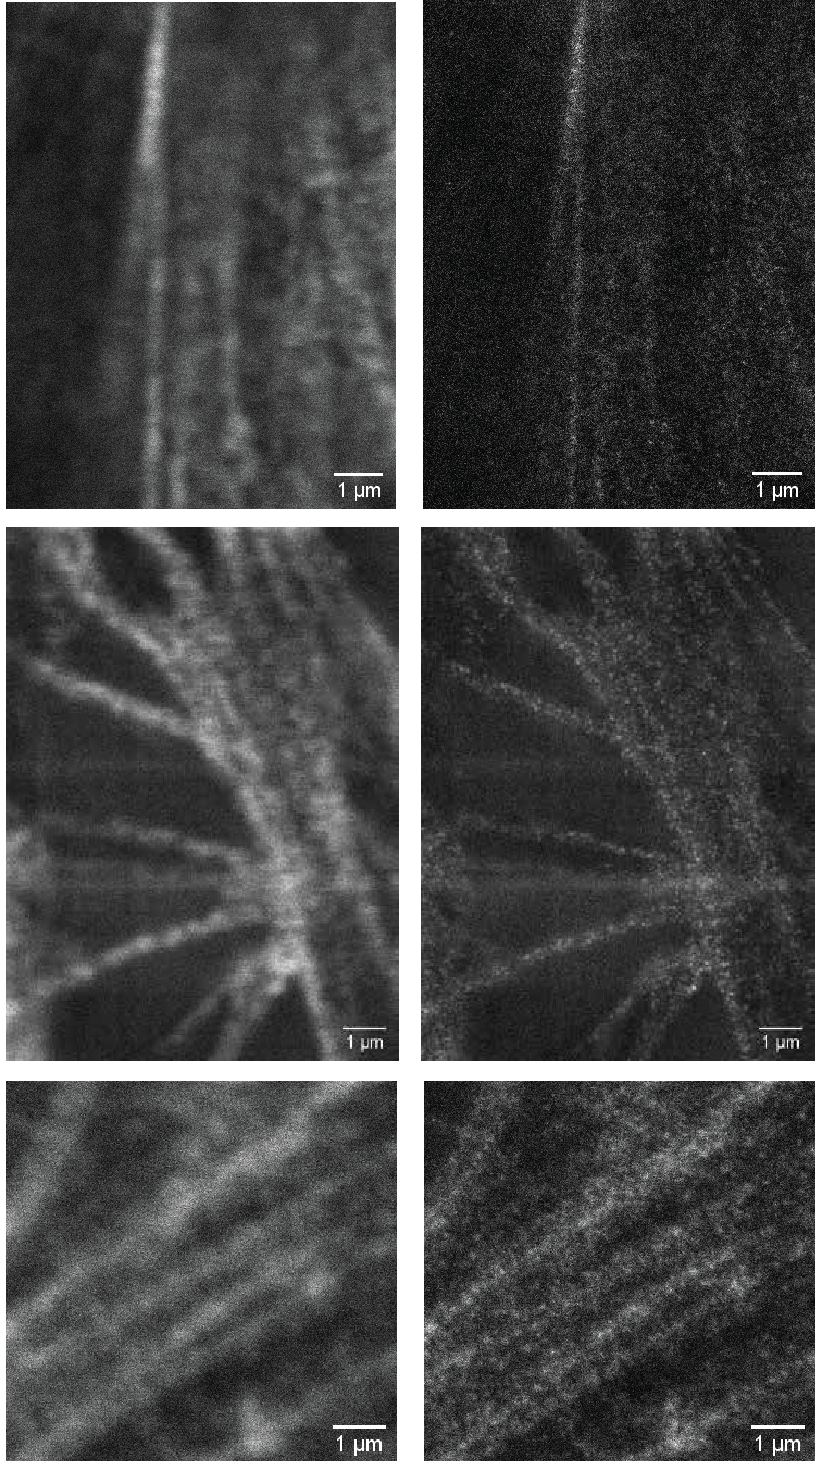
\includegraphics[width=.8\linewidth]{ssted_1.pdf}
	\caption{
		Confocal (left) and STED (right) acquisitions of various fields of view.
	}
	\label{fig:ssted supplementary}
\end{figure}


\begin{figure}
	\centering
	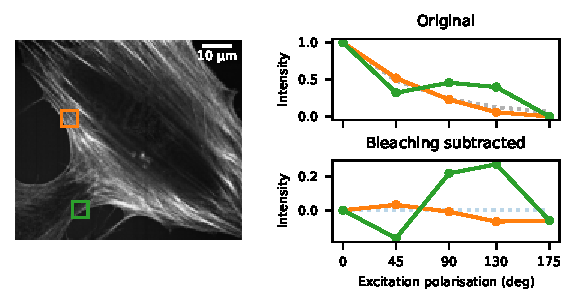
\includegraphics{ssted_pol.pdf}
	\caption{
		\textbf{Left:} First frame of a polarisation acquisition series, with two ROIs indicated that contain fibres of roughly perpendicular orientation. \textbf{Top right:} Integrated intensity of those ROIs at different sample points, normalised to the intensity present in the first frame. Dashed line: best-fit exponential curve. \textbf{Bottom right:} Same as top right, but with the exponential subtracted.
	}
	\label{fig:ssted pol}
\end{figure}

Even though using polarisation on the detection side is still impossible, the setup is able to obtain polarisation-resolved images by varying the angle of excitation polarisation. As a proof of concept, the sample described in \autoref{sec:samples} was imaged with linearly polarised excitation light from \ang{0} to \ang{170} in steps of \ang{10}. Applying the algorithm detailed in \autoref{sec:pol analysis} to three different ROIs resulted in \autoref{fig:composite}. As expected, vertically oriented fibres are excited by horizontal polarisation, because the transition dipole of SiR-actin is more or less orthogonal to the fibre \cite{Spira2017}.
A power-law scaling of the saturation (degree of polarisation) and value (total brightness) in the algorithm can be used to adjust the brightness and contrast of the figure, as shown in \autoref{fig:power law exponents}.

\begin{figure}
	\centering
	\newlength{\spacing}
	\setlength{\spacing}{7pt}
	
	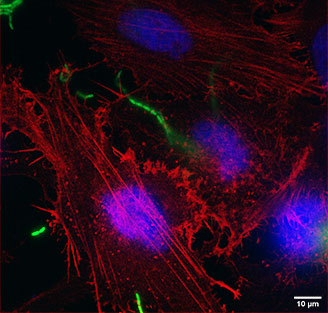
\includegraphics[height=.47\linewidth]{composite.jpg}%
	\hspace{\spacing}%
	\includegraphics[height=.47\linewidth]{conventional_pol_0_scalebar.png}
	
	\vspace{\spacing}
	
	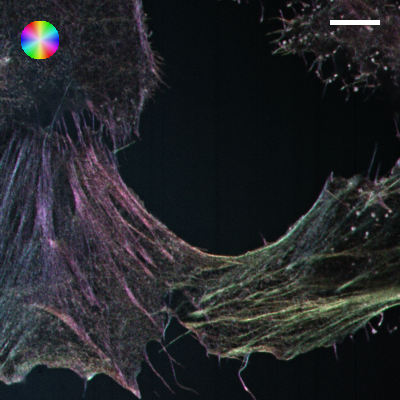
\includegraphics[height=.47\linewidth]{conventional_pol_1.png}%
	\hspace{\spacing}%
	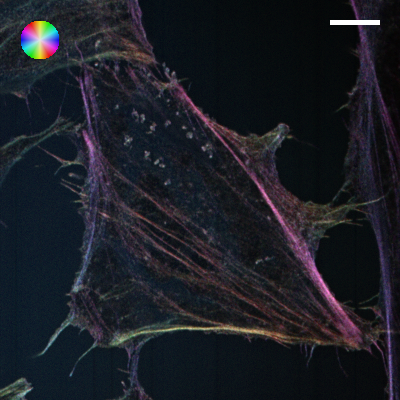
\includegraphics[height=.47\linewidth]{conventional_pol_2.png}
	
	\caption{
		\textbf{Top left:} Composite view of a Yersinia sample, labelled with phalloidin instead of actin. Blue: DNA (DAPI). Green: bacteria (GFP). Red: actin (phalloidin).
		\textbf{Others:} Polarisation microscopy images of three different cells. The colour wheel indicates the direction of polarised light corresponding to a certain colour. Scale bars \SI{10}{\mu m}.
	}
	\label{fig:composite}
\end{figure}

\begin{figure}
	\centering
	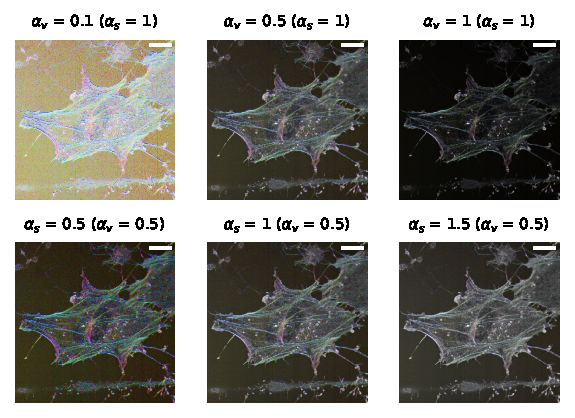
\includegraphics{conventional_pol.pdf}
	\caption{
		The effect of the exponents $ \alpha_s $ (tuning saturation) and $ \alpha_v $ (scaling brightness) on an image.
	}
	\label{fig:power law exponents}
\end{figure}

Polarisation images at STED resolution are unfortunately difficult to acquire due to strong photobleaching, which limits the number of points at which the excitation polarisation can be sampled (see \autoref{fig:ssted pol}). There is a qualitative difference between the intensity profile of two ROIs that contain orthogonally oriented actin fibres. In particular, the maximum of one is located at \ang{45} (after subtracting an exponential photobleaching response), while the other shows a maximum around \ang{135}. The quality of this particular image is unfortunately not sufficient to colour it as in \autoref{fig:composite}.

In short, this section demonstrates successful conventional polarisation microscopy on the microscope setup and that SiR-actin is a suitable fluorophore to conduct research in Yersinia samples. There are two main limitations at the moment: the detection waveplates are not calibrated correctly, so using polarisation in the detection pathway is impossible, and the trade-off between spatial resolution and polarisation information requires special care.


\section{pSTED}

Because the microscope was not set up to enable control over the polarisation of the depletion laser, a set of two new waveplates had to be installed to achieve polarisation-dependent depletion at the sample. A QWP was installed to negate the effects of the HWP and the QWP at the microscope end of the optical enclosure, and a HWP to control the polarisation angle. More details are presented in \autoref{sec:psted implementation}.

After setting up the pSTED optics, these are the results so far: to verify that stimulated emission is polarisation-dependent, isotropic fluorescent beads were exposed to two different conditions. In the first condition, the beads were excited with vertically polarised light and depleted by a laser polarised along different angles and at different power levels. Regardless of the angle, the fluorescence signal drops as the depletion power is increased, but the rate at which depends on the depletion polarisation. The depletion rate is highest when the lasers are aligned and lowest when they are orthogonal. This result can be explained by photoselection. When an isotropic sample is excited by linearly polarised light, fluorophores with a dipole moment orthogonal to the excitation beam will not be excited. As a result, the average excited fluorophore's transition dipole is oriented parallel to the excitation polarisation. Since depletion is most effective when the depletion polarisation is aligned with the fluorophore (as predicted by \autoref{eq:psted integral}) in this case that also means it is most effective when aligned with the excitation laser. This was indeed observed, see \autoref{fig:psted beads} (Left). 

On the other hand, if the sample is excited with circularly polarised light, the rate of depletion should not depend on the depletion polarisation. This measurement was performed twice. The first time by imaging an ROI at different depletion powers before changing the depletion polarisation and the second time by imaging ROIs at different depletion polarisations before changing the depletion power. The average of those measurements is shown in \autoref{fig:psted beads} (Right). While the results are substantially different from the linear polarisation case, it has not been calculated whether the difference between them is statistically significant. This would be an important calculation to do. (Note that it was much easier to automate the acquisition of the linear polarisation data. As such, the figure shown is an average of five runs, while the other only shows data of a single run.)

\begin{figure}
	\centering
	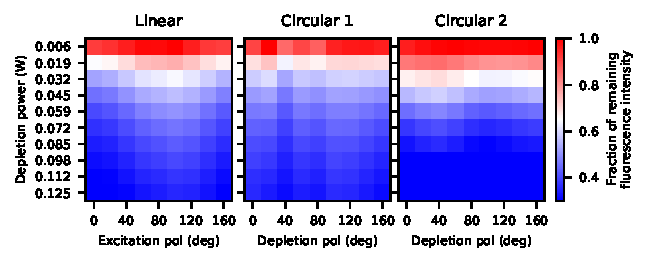
\includegraphics{psted_beads.pdf}
	\caption{
		Dependency of surviving fluorescence on intensity and polarisation of depletion beam. \textbf{Left:} linearly polarised excitation at 0° (vertical). \textbf{Right:} circularly polarised excitation.
	}
	\label{fig:psted beads}
\end{figure}

Even though they could be improved, the results do show that depletion efficiency seems to be dependent on the polarisation of the depletion laser and the orientation of the fluorophore, and that pSTED is likely to work. Another experiment was performed on a cell sample, but since the actin fibres are not isotropic, it was unnecessary to use linearly polarised excitation to select a subset of fluorophores. Instead, several fibres were imaged with circularly polarised excitation light and manipulated the depletion angle to assess whether it was possible to perform pSTED on a biological sample, see \autoref{fig:psted scans}. Without a depletion laser, photobleaching is visible (blue). With a depletion laser, the photobleaching response disappears and is taken over by a signal that depends on the depletion polarisation (orange). Although more research is needed, this shows that pSTED could be a valuable new tool in the polarisation microscopy field.

\begin{figure}
	\centering
	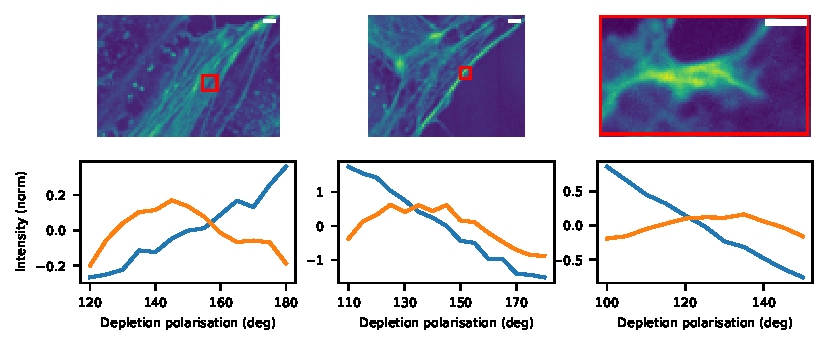
\includegraphics{psted_scans.pdf}
	\caption{
		When samples are excited with circularly polarised light, the polarisation of the depletion beam can modulate the fluorescence intensity. \textbf{Top:} FOVs with a marked ROI in red. \textbf{Bottom:} Intensity profile, as a function of depletion polarisation. Orange: depletion beam turned on. Blue: depletion beam turned off.
	}
	\label{fig:psted scans}
\end{figure}




























